\section{Convolution and GEMM}
\label{sec:background}

Convolution takes three input tensors: the input image, filters, and output (illustrated in \rfig{tensors}), along with an optional bias array. 
These four-dimensional tensors can have different data layouts, that is, the order in which their dimensions are stored in memory. 
In addition to the input tensors, convolution utilizes several parameters defined in \rtab{conv-parameters} that modify its behavior. 

\begin{table}[t]
    \caption{Notation for convolution parameters.}
    \label{tab:conv-parameters}
    \small
    \centering
    \begin{tabular}{ll|ll}
    \texttt{N}:  & Batch size       & \texttt{IC}: & Input channels   \\ \hline
    \texttt{IH}: & Input height     & \texttt{IW}: & Input width      \\ \hline
    \texttt{OC}: & Output channels  & \texttt{OH}: & Output height    \\ \hline
    \texttt{OW}: & Output width     & \texttt{FH}: & Filter height    \\ \hline
    \texttt{FW}: & Filter width     & \texttt{SH}: & Stride height    \\ \hline
    \texttt{SW}: & Stride width     & \texttt{DH}: & Dilation height  \\ \hline
    \texttt{DW}: & Dilation width   & \texttt{PH}: & Padding height   \\ \hline
    \texttt{PW}: & Padding width    & \texttt{GR}: & Groups           
    \end{tabular}
\end{table}

\begin{figure}[t]
    \centering
    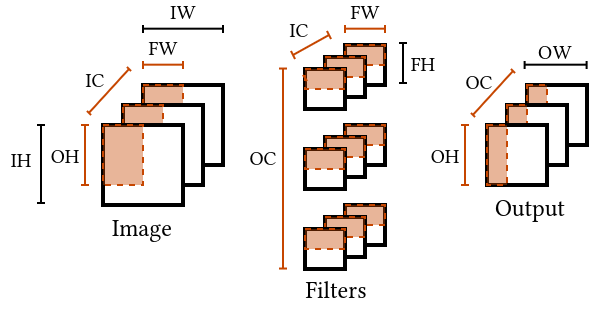
\includegraphics[width=0.85\columnwidth]{figures/zconv-gemm-column.png}
    % \Description{Three tensors. An IH by IW by IC image, a OC by IC by FH by FW filter, and a OH by OW by OC output.}
    \caption{Convolution tensors and their respective dimensions (omitting batch).
    Highlighted in orange, an example of the inputs for a GEMM call within \algname.}
    \label{fig:tensors}
\end{figure}

GEMM is defined in \eqref{eq:gemm}, where $\alpha$ and $\beta$ are scalar values, and $C_{m \times n}$, $A_{m \times k}$, and $B_{k \times n}$ are the matrix operands.
This API uses the following parameters:
\begin{enumerate*}[label=(\roman*)] 
    \item \emph{layout}: the memory layout of matrices (row-major or column-major), 
    \item \emph{trans{x}}: whether to transpose matrix \emph{x} before multiplication, 
    \item \emph{m}, \emph{n}, \emph{k}: the dimension sizes of the matrices,
    \item \emph{alpha} and \emph{beta}: the scalar multiplier parameters,
    \item \emph{ld{x}}: the leading dimension for matrix \emph{x}.
    For row-major matrices, \emph{ld{x}} is the number of elements in memory between consecutive rows,
    \item \emph{a}, \emph{b}, \emph{c}: the base pointers to the matrices.
\end{enumerate*}

\begin{equation}
    \label{eq:gemm}
    C_{m \times n} = \beta C_{m \times n} + \alpha A_{m \times k} \cdot B_{k \times n}
\end{equation}

While the Im2col approach transforms the convolution input image into a new contiguous matrix, the GEMM API supports non-contiguous input matrices.
In the row-major layout, the GEMM API only assumes that elements within a row are contiguous.
The stride between rows, the row size, and the starting position of the matrix are all flexible and configurable through the parameters previously mentioned.
The column-major layout operates similarly, but with contiguous columns instead of rows.
BLAS libraries rely on tiling—dividing input matrices into smaller submatrices (tiles)—and packing matrices into contiguous buffers to optimize cache locality~\cite{Goto2008,Rohwedder2023}.
These transformations also allow GEMM to achieve high performance with non-contiguous inputs.
\algname leverages GEMM's API flexibility by providing non-contiguous matrices directly to GEMM.